\documentclass[a4paper]{article}
\usepackage{amsmath}
\usepackage{amssymb}
\usepackage{xcolor}
\usepackage{amsthm}
\usepackage{dsfont}
\usepackage{graphicx}
\usepackage{hyperref}
\usepackage{datetime}
\usepackage{outlines}
\usepackage{float}
\usepackage{booktabs}
\usepackage{enumitem}
\usepackage{sidecap}

% link coloring
%\hypersetup{
%    colorlinks,
%    linkcolor={red!80!black},
%    citecolor={green!60!black},
%    urlcolor={blue!80!black}
%}

% end of proof symbol
\newcommand{\newmarkedtheorem}[1]{%
  \newenvironment{#1}
    {\pushQED{\qed}\csname inner@#1\endcsname}
    {\popQED\csname endinner@#1\endcsname}%
  \newtheorem{inner@#1}%
}

\theoremstyle{definition}
%\newtheorem{eg}{Example}[section]
\newmarkedtheorem{eg}{Example}[section]
\newtheorem{observation}{Observation}[section]
\newtheorem{define}{Definition}[section]
\theoremstyle{plain}
\newtheorem{proposition}{Proposition}
\newtheorem{lemma}{Lemma}
\newtheorem{corollary}{Corollary}
\newtheorem{theorem}{Theorem}[section]
\newtheorem{assump}{Assumption}
\newtheorem{remark}{Remark}

\newdateformat{monthyeardate}{\monthname[\THEMONTH] \THEYEAR}

\author{Jeroen van Riel}
\date{\monthyeardate\today}
\title{Trajectory Optimization}


\begin{document}



\section*{Single intersection}

\begin{SCfigure}
  \centering
  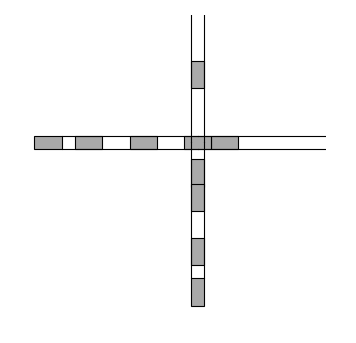
\includegraphics[width=0.4\textwidth]{figures/single_intersection_example.png}
  \caption{Illustration of a single intersection with vehicles drawn as grey
    rectangles. Vehicles approach the intersection from the east and from the
    south and cross it without turning. Note that the first two waiting vehicles
    on the south lane kept some distance before the intersection, such that they
    are able to reach full speed whenever they
    cross.}\label{fig:intersection_illustration}
\end{SCfigure}

We are interested in algorithms to efficiently control the movement of vehicles
through a network of intersections under safety constraints. In order to keep
the problem simple, we assume that vehicle routes are fixed and known whenever a
vehicle enters the network. This means that we can consider the longitudinal
position $x_{i}(t)$ of each vehicle $i$ along its route, for which we use the
well-known \textit{double integrator} model
\begin{gather}
  \label{eq:vehicle_dynamics}
\begin{aligned}
  \dot{x}_{i}(t) = v_{i}(t) , \\
  \dot{v}_{i}(t) = u_{i}(t)  , \\
  0 \leq v_{\max} \leq v_{\max} , \\
  |u_{i}(t) | \leq a_{\max} ,
\end{aligned}
\end{gather}
where $v_{i}(t)$ is the vehicle's velocity and $u_{i}(t)$ its acceleration,
which is set by the controller. Let $D_{i}(s_{i,0})$ denote the set of all
trajectories $x_{i}(t)$ satisfying these
dynamics, given some initial state $s_{i,0} = (x_{i}(0), v_{i}(0))$.

Before we consider networks of intersections, we first state the problem for a
single intersection as illustrated in Figure~\ref{fig:intersection_illustration}. Assume there are two incoming
lanes, identified by indices $\mathcal{R} = \{ 1, 2 \}$. The corresponding two
routes are crossing the intersection from south to north and crossing from west
to east. We identify vehicles by their route and by their relative order on this
route, by defining the vehicle index set
\begin{align}
  \mathcal{N} = \{ (r, k) : k \in \{1, \dots, n_{r}\}, r \in \mathcal{R}\} ,
\end{align}
where $n_{r}$ denotes the number of vehicles following route $r$. Smaller
values of $k$ correspond to being closer to the intersection. Given vehicle
index $i = (r, k) \in \mathcal{N}$, we also use the notation $r(i) = r$ and
$k(i) = k$.
%
We assume that each vehicle is represented as a rectangle of length $L$ and
width $W$ and that $x_{i}(t)$ is measured at the front bumper. In order to
maintain a safe distance between consecutive vehicle on the same lane, vehicle
trajectories need to satisfy
\begin{align}
  \label{eq:follow_constraints}
  x_{i}(t) - x_{j}(t) \geq L ,
\end{align}
for all $t$ and all pairs of indices $i, j \in \mathcal{N}$ such that
$r(i) = r(j), k(i) + 1 = k(j)$. Let $\mathcal{C}$ denote the set of such ordered
pairs of indices. Note that these constraints restrict vehicle from overtaking
each other, so the initial relative order is always maintained.
%
For each $i \in \mathcal{N}$, let $\mathcal{E}_{i} = (B_{i}, E_{i})$ denote the
open interval such that vehicle $i$ occupies the intersection's conflict area if
and only if $B_{i} < x_{i}(t) < E_{i}$. Using this notation, collision avoidance
at the intersection is achieved by requiring
\begin{align}
  \label{eq:conflict_constraints}
  (x_{i}(t), x_{j}(t)) \notin \mathcal{E}_{i} \times \mathcal{E}_{j} ,
\end{align}
for all $t$ and for all pairs of indices $i, j \in \mathcal{N}$ with
$r(i) \neq r(j)$, which we collect in the set $\mathcal{D}$.
%
Suppose we have some performance criterion $J(x_{i})$ that takes into account
travel time and energy efficiency of the trajectory of vehicle $i$, then the
offline trajectory optimization problem for a single intersection can be
compactly written as
\begin{subequations}
\label{eq:offline_single_intersection}
\begin{align}
  \min_{\mathbf{x}(t)} \quad & \sum_{i \in \mathcal{N}} J(x_{i}) \\
  \text{s.t.} \quad  & x_{i} \in D_{i}(s_{i,0}) , &\text{for all } i \in \mathcal{N} , \\
                & x_{i}(t) - x_{j}(t) \geq L, &\text{for all } (i,j) \in \mathcal{C} , \\
                & (x_{i}(t), x_{j}(t))  \notin \mathcal{E}_{i} \times \mathcal{E}_{j} , &\text{for all } \{i,j\} \in \mathcal{D} \label{eq:collision_constraints} ,
\end{align}
\end{subequations}
where $\mathbf{x}(t) = [\, x_{i}(t) : i \in \mathcal{N} \,]$ and constraints are
for all $t$.

\subsection*{Direct transcription}

Although computationally demanding,
problem~\eqref{eq:offline_single_intersection} can be numerically solved by
direct transcription to a non-convex mixed-integer linear program by
discretization on a uniform time grid. Let $K$ denote the number of discrete
time steps and let $\Delta t$ denote the time step size.
%
Using the forward Euler integration scheme, we have
\begin{align*}
  x_{i}(t + \Delta t) = x_{i}(t) + v_{i}(t) \Delta t , \\
  v_{i}(t + \Delta t) = v_{i}(t) + u_{i}(t) \Delta t ,
\end{align*}
for each $t \in \{0, \Delta t, \dots, K \Delta t\}$. Following the approach
in~\cite{hultApproximateSolutionOptimal2015}, the collision-avoidance
constraints between lanes can be formulated using the well-known big-M technique
by the constraints
\begin{align*}
  x_{i}(t) \leq B_{i} + \delta_{i}(t) M , \\
  E_{i} - \gamma_{i}(t) M \leq x_{i}(t) , \\
  \delta_{i}(t) + \delta_{j}(t) + \gamma_{i}(t) + \gamma_{j}(t) \leq 3 ,
\end{align*}
where $\delta_{i}(t), \gamma_{i}(t) \in \{ 0, 1 \}$ for all $i \in \mathcal{N}$ and $M$ is a
sufficiently large number.
%
Finally, the follow constraints can simply be added as
\begin{align*}
  x_{i}(t) - x_{j}(t) \geq L ,
\end{align*}
for each $t \in \{0, \Delta t, \dots, K \Delta t\}$ and each pair of consecutive
vehicles $(i, j) \in \mathcal{C}$ on the same lane.
%
For example, consider the objective functional
\begin{align*}
  J(x_{i}) = \int_{t=0}^{t_{f}} \left( {(v_{d} - v_{i}(t))}^{2} + {u_{i}(t)}^{2} \right) dt ,
\end{align*}
where $v_{d}$ is some reference velocity and $t_{f}$ denotes the final time,
then the optimal trajectories are shown in
Figure~\ref{fig:direct_transcription_example}.

\begin{table}[H]
  \centering
\begin{tabular}{ c | c c c | c c }
  $i$  & (1,1) & (1,2) & (1,3) & (2,1) & (2,2) \\
  \hline
  $x_{i}(0)$ & 15 & 10 &  0 & 10 &  0 \\
  $v_{i}(0)$ & 10 & 10 & 10 & 10 & 10 \\
\end{tabular}
\caption{Example initial conditions $s_{i,0} = (x_{i}(0), v_{i}(0))$ for
  problem~\eqref{eq:offline_single_intersection}.}
\label{tab:hult_parameters}
\end{table}

\begin{figure}[t]
  \centering
  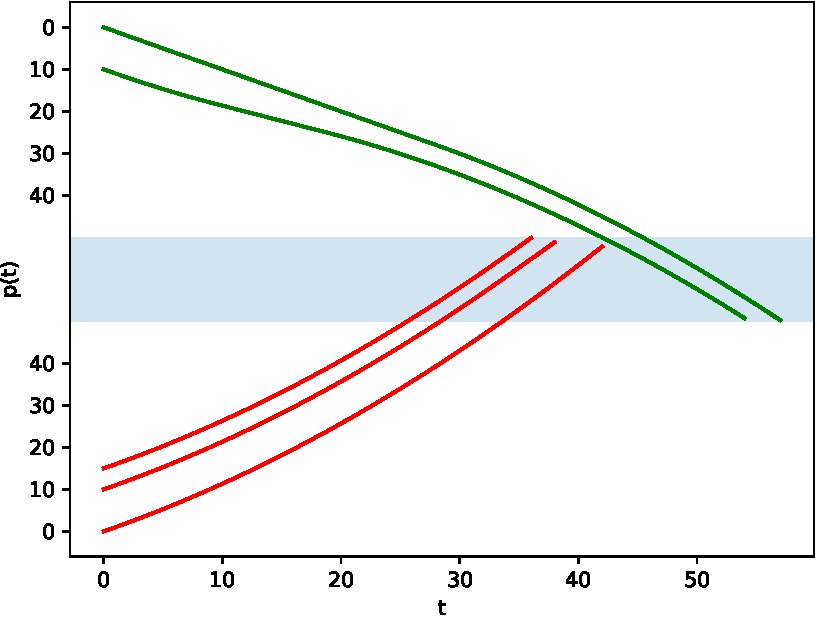
\includegraphics[width=0.7\textwidth]{figures/direct_transcription_example.pdf}
  \caption{Example of optimal trajectories obtained using the direct
    transcription method with
    $L = 5, \, \mathcal{E}_{i} \equiv \mathcal{E} = [50, 70], \, v_{d} = 20, \; T=120, \, \Delta t = 0.1$
    and initial conditions as given in Table~\ref{tab:hult_parameters}. The
    y-axis is split such that each part corresponds to one of the two lanes and
    the trajectories are inverted accordingly and drawn with separate colors.
    The intersection area $\mathcal{E}$ is drawn as a shaded region. Whenever a
    vehicle has left the intersection, we stop drawing its trajectory for
    clarity.}
  \label{fig:direct_transcription_example}
\end{figure}


\subsection*{Occupancy time slots}

For the case where only a single vehicle is approaching the intersection for
each route, so $n_{r} = 1$ for each route $r \in \mathcal{R}$, it has been shown
that problem~\eqref{eq:offline_single_intersection} can be decomposed into two coupled optimization problems, see
Theorem 1 in~\cite{hultApproximateSolutionOptimal2015}. Roughly speaking, the \textit{upper-level problem} optimizes the time
slots during which vehicles occupy the intersection, while the \textit{lower-level problem}
produces optimal safe trajectories that respect these time slots.
%
When allowing multiple vehicles per lane, we show without proof that a similar
decomposition is possible.
%
Given $x_{i}(t)$, the \textit{crossing time} of vehicle $i$, when the vehicle
first enters the intersection, and the corresponding \textit{exit time} are respectively
\begin{align}
  \inf \{ t: x_{i}(t) \in \mathcal{E}_{i} \}  \; \text{ and } \; \sup \{ t: x_{i}(t) \in \mathcal{E}_{i} \} .
\end{align}
%
The upper-level problem is to find a set of feasible occupancy timeslots, for
which the lower-level problem generates trajectories. We will use decision
variable $y(i)$ for the crossing time and write $y(i) + \sigma(i)$ for the exit
time. It turns out that trajectories can be generated separately for each route,
which yields the decomposition
%
\begin{subequations}
\begin{align}
  \min_{y, \sigma} \quad & \sum_{r \in \mathcal{R}} F(y_{r}, \sigma_{r}) \\
  \text{ s.t. } \quad & y(i) + \sigma(i) \leq y(j) \text{ or } y(j) + \sigma(j) \leq y(i), & \text{ for all } (i, j) \in \mathcal{D} , \\
  & (y_{r}, \sigma_{r}) \in \mathcal{S}_{r} , & \text{ for all } r \in \mathcal{R} ,
\end{align}
\end{subequations}
where $F(y_{r}, \sigma_{r})$ and $\mathcal{S}_{r}$ are the value function and
set of feasible parameters, respectively, of the lower-level \textit{route trajectory optimization}
problem
\begin{subequations}
\begin{align}
  F(y_{r}, \sigma_{r}) = \min_{x_{r}} \quad & \sum_{i \in \mathcal{N}(r)} J(x_{i}) \\
  \text{ s.t. } \quad & x_{i} \in D_{i}(s_{i,0}) , & \text{ for all } i \in \mathcal{N}_{r} , \\
  & x_{i}(y(i)) = B_{i} , & \text{ for all } i \in \mathcal{N}_{r} , \\
  & x_{i}(y(i) + \sigma(i)) = E_{i} , & \text{ for all } i \in \mathcal{N}_{r} , \\
  & x_{i}(t) - x_{j}(t) \geq L , & \text{ for all } (i, j) \in \mathcal{C} \cap \mathcal{N}_{r} ,
\end{align}
\end{subequations}
where we used $\mathcal{N}_{r} = \{ i \in \mathcal{N} : r(i) = r \}$ and
similarly for $x_{r}, y_{r}$ and $\sigma_{r}$ to group variables according to
route. Note that the set of feasible parameters $\mathcal{S}_{r}$ implicitly
depends on the initial states $s_{r}$ and system parameters.


\subsection*{Delay objective}

Assume that the trajectory performance criterion is exactly the crossing time,
so $J(x_{i}) = \inf \{ t: x_{i}(t) \in \mathcal{E}_{i} \}$. This assumption
makes the problem significantly easier, because we have
\begin{align}
  F(y_{r}, \sigma_{r}) \equiv F(y_{r}) = \sum_{i \in \mathcal{N}_{r}} y(i) .
\end{align}
%
Furthermore, we assume that vehicles enter the network and cross the
intersection at full speed, so $v_{i}(0) = v_{i}(y(i)) = v_{\max}$, such that we
have
\begin{align}
\sigma(i) \equiv \sigma = (L + W) / v_{\max}, \; \text{ for all } i \in \mathcal{N} .
\end{align}
%
Therefore, we ignore the part related to $\sigma$ in the set of feasible
parameters $\mathcal{S}_{r}$, which can be shown that to have a particularly
simple structure under these assumptions.
% earliest time of arrival
Observe that $r_{i} = (B_{i} - x_{i}(0)) / v_{\max}$ is the earliest time at
which vehicle $i$ can enter the intersection.
%
Let $\rho = L / v_{\max}$ be such that $y(i) + \rho$ is the time at which
the rear bumper of a crossing vehicle reaches the start line of the
intersection, then it can be shown that
$y_{r} \in \mathcal{S}_{r}$ whenever
\begin{subequations}
\begin{align}
  r_{i} \leq y(i) , & \text{ for all } i \in \mathcal{N}_{r} , \\
  y(i) + \rho \leq y(j) , & \text{ for all } (i,j) \in \mathcal{C} \cap \mathcal{N}_{r} .
\end{align}
\end{subequations}
Therefore, under the stated assumptions,
problem~\eqref{eq:offline_single_intersection} reduces to the following \textit{crossing time scheduling} problem
\begin{subequations}
\begin{align}
  \min_{y} \quad & \sum_{i \in \mathcal{N}} y(i) \\
  \text{ s.t. } \quad & r_{i} \leq y(i) , & \text{ for all } i \in \mathcal{N} , \\
                    & y(i) + \rho \leq y(j) , & \text{ for all } (i,j) \in \mathcal{C} , \\
                    & y(i) + \sigma \leq y(j) \text{ or } y(j) + \sigma \leq y(i) , & \text{ for all } (i,j) \in \mathcal{D} \label{eq:disjunctive} ,
\end{align}
\end{subequations}
which can be solved using off-the-shelf mixed-integer linear program solvers,
after encoding the \textit{disjunctive constraints}~\eqref{eq:disjunctive} using the big-M
technique. Given optimal $y^{*}$, any set of trajectories
$[x_{i}(t) : i \in \mathcal{N}]$ that satisfies
\begin{subequations}
\begin{align}
  x_{i} \in D_{i}(s_{i,0}) , \quad & \text{ for all } i \in \mathcal{N} , \\
  x_{i}(y^{*}(i)) = B_{i} , \quad & \text{ for all } i \in \mathcal{N} , \\
  x_{i}(y^{*}(i) + \sigma) = E_{i} , \quad & \text{ for all } i \in \mathcal{N} , \\
  x_{i}(t) - x_{j}(t) \geq L , \quad & \text{ for all } (i,j) \in \mathcal{C} ,
\end{align}
\end{subequations}
forms a valid solution. We show how these trajectories can be computed by an
efficient direct transcription method. First of all, note that each route may be
considered separately and trajectories can be computed in a sequential fashion
by repeatedly solving the optimal control problem
%
\begin{align*}
\texttt{MotionSynthesize}(\tau, B, s_{0}, x') := \\
  {\arg\min}_{x: [0, \tau] \rightarrow \mathbb{R}} & \int_{0}^{\tau} |x(t)| dt \\
  \text{ s.t. } & \ddot{x}(t) = u(t) , &  \text{ for all } t \in [0, \tau] , \\
  & |u(t)| \leq a_{\max} , &  \text{ for all } t \in [0, \tau] , \\
  & 0 \leq \dot{x}(t) \leq v_{\max} , &  \text{ for all } t \in [0, \tau] , \\
  & x'(t) - x(t) \geq L , &  \text{ for all } t \in [0, \tau] , \\
  & (x(0), \dot{x}(0)) = s_{0} , \\
  & (x(\tau), \dot{x}(\tau)) = (B, v_{\max}) ,
\end{align*}
where $\tau$ is set to the required crossing time, $B$ denotes the distance to
the intersection, $s_{0}$ is the initial state of the vehicle and $x'$ denotes
the trajectory of the vehicle preceding the current vehicle.


\newpage

\section*{Trajectories in networks}

\begin{SCfigure}
  \centering
  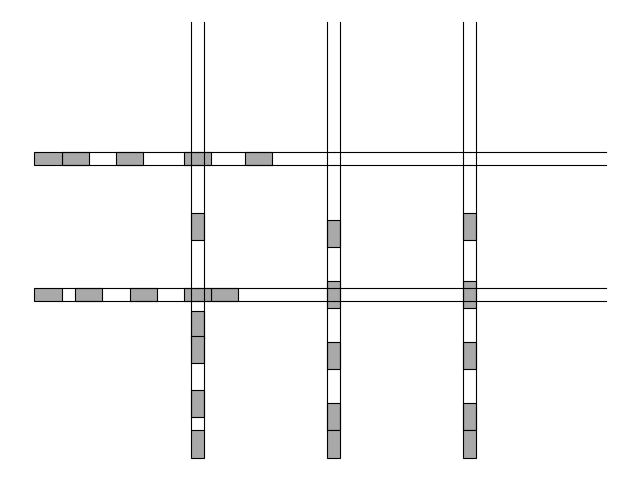
\includegraphics[width=0.55\textwidth]{figures/state_example.png}
  \caption{Illustration of some grid-like network of intersections with vehicles
    drawn as grey rectangles. There are five vehicle routes: two from east to
    west and three from south to north. Turning at intersections is not
    allowed.}\label{fig:network_illustration}
\end{SCfigure}

To extend the model to a network of intersections, illustrated in Figure~\ref{fig:network_illustration}, we
need some additional notation to encode the network topology.
% network definition
We define a directed graph $(V,E)$ with nodes $V$ and arcs $E$, representing the
possible paths that vehicles can follow. Nodes of in-degree at least two are
called \textit{intersections}. Nodes with only outgoing arcs are
\textit{entrypoints} and nodes with only incoming arcs are \textit{exitpoints}.
%
Let $d(v, w)$ denote the distance between nodes $v$ and $w$.
%
For each route index $r \in \mathcal{R}$, we let
\begin{align}
  \bar{V}_{r} = (v_{r}(0), v_{r}(1), \dots, v_{r}(m_{r}), v_{r}(m_{r+1}))
\end{align}
be the path that vehicles $i \in \mathcal{N}_{r}$ follow through the network. We
require that the first node $v_{r}(0)$ is an entrypoint and that the last node
$v_{r}(m_{r+1})$ is an exitpoint and we write
\begin{align}
  V_{r} = \bar{V}_{r} \setminus \{ v_{r}(0), \, v_{r}(m_{r+1}) \}
\end{align}
to denote the path restricted to intersections. We write $(v, w) \in V_{r}$ for
some $(v, w) \in E$ whenever $v$ and $w$ are two consecutive nodes on the path.
We require that routes can only overlap at nodes by making the following assumption.

\begin{assump}\label{assump:disjoint_routes}
  Every arc $(v,w) \in E$ is part of at most one route $V_{r}$.
\end{assump}

Assume that physical lanes are axis-aligned and that routes are such that no
turning is required. For each $v \in V_{r}$ define the conflict zone
$\mathcal{E}_{r}(v) = (B_{r}(v), E_{r}(v))$ and consider the union
\begin{align}
  \mathcal{E}_{r} = \bigcup_{v \in V_{r}} \mathcal{E}_{r}(v)
\end{align}
corresponding to the positions of vehicles $i \in \mathcal{N}_{r}$ for which it
occupies an intersection on its path $V_{r}$.
%
By reading $\mathcal{E}_{i} \equiv \mathcal{E}_{r}$ for $r(i) = r$, the single
intersection problem~\eqref{eq:offline_single_intersection} naturally extends to
the network case. Like before, the resulting problem can be numerically solved
by a direct transcription method.
%
The natural extension of the two-stage decomposition is to solve the occupancy time scheduling problem
\begin{subequations}
\begin{align}
  \min_{y,\sigma} \;\; & \sum_{r \in \mathcal{R}} F(y_{r}, \sigma_{r}) \\
  \text{ s.t. } & y(i,v) + \sigma(i,v) \leq y(j,v) \text{ or }  \\
                & y(j,v) + \sigma(j,v) \leq y(i,v) , & \text{ for all } \{i,j\} \in \mathcal{D}^{v} \text{ and } v \in V, \\
  & (y_{r}, \sigma_{r}) \in \mathcal{S}_{r} , \quad & \text{ for all } r \in \mathcal{R} ,
\end{align}
\end{subequations}
where the set of conflict pairs at node $v$ is defined as
\begin{align}
\mathcal{D}^{v} = \{ \{i,j\} \subset \mathcal{N} : r(i) \neq r(j), v \in V_{r(i)} \cap V_{r(j)} \} ,
\end{align}
%
where $F(y_{r}, \sigma_{r})$ and $\mathcal{S}_{r}$ are the value function and
set of feasible parameters, respectively, of the parametric trajectory
optimization problems
%
\begin{subequations}
\begin{align}
  F(y_{r}, \sigma_{r}) = \min_{x_{r}} & \; \sum_{r \in \mathcal{R}} J(x_{i}) \\
  \text{ s.t. } & x_{i}(t) \in D_{i}(s_{i,0}) , \quad & \text{ for } i \in \mathcal{N}_{r} , \\
  & x_{i}(y(i,v)) = B_{r}(v) , \quad & \text{ for } v \in V_{r} , i \in \mathcal{N}_{r} , \\
  & x_{i}(y(i,v) + \sigma(i,v)) = E_{r}(v) , \quad & \text{ for } v \in V_{r} , i \in \mathcal{N}_{r} , \\
  & x_{i}(t) - x_{j}(t) \geq L , \quad & \text{ for } (i, j) \in \mathcal{C} \cap \mathcal{N}_{r} .
\end{align}
\end{subequations}


\subsection*{Delay objective}

Suppose we use use the crossing at the last intersection as performance measure, by defining the
objective function as
\begin{align}
  J(x_{i}) = \inf \{ t: x_{i}(t) \in \mathcal{E}_{r}(v_{r}(m_{r}))\} .
\end{align}
%
We show how to reduce the resulting problem to a scheduling problem, like we did
in the single intersection case.
%
Again, we require vehicles to drive at full speed whenever they occupy any
intersection such that $\sigma_{i} \equiv \sigma = (L + W) / v_{\max}$.
%
For each $r \in \mathcal{R}$, we provide a sufficient set of constraints on the
crossing times
\begin{align}
y(i, v) = \inf \{ t: x_{i}(t) \in \mathcal{E}_{r}(v) \}
\end{align}
such that the corresponding lower-level problems are feasible, which we write as
$y_{r} \in \mathcal{S}_{r}$, so we let $r \in \mathcal{R}$ be an arbitrary route
in the following discussion.
%
Like for the single intersection,
let $\rho = L / v_{\max}$ denote the minimum time between two crossing times of
vehicles of the same class.
%
First of all, vehicles of the same class are required to keep safe distance, so we need
\begin{align}
  \label{eq:conjunctive_constraints}
  y(i, v) + \rho \leq y(j, v) , \quad \text{ for all } (i,j) \in \mathcal{C} \text{ and } v \in V.
\end{align}
%
Assuming that the initial velocity satisfies
$v_{i}(0) = v_{\max}$, we require
\begin{align}
  \label{eq:release_constraints}
r_{i} = (B_{r(i)}(v_{r}(l)) - x_{i}(0)) / v_{\max} \leq y(i, v_{r}(l)) ,
\end{align}
where $l$ is the smallest integer such that
$x_{i}(0) \leq B_{r(i)}(v_{r}(l))$.
%
For every $(v, w) \in V_{r}$, we require the \textit{travel constraint}
\begin{align}
  \label{eq:travel_constraints}
  y(i, v) + d(v, w) / v_{\max} \leq y(i, w)
\end{align}
for every $i \in \mathcal{N}_{r}$ to model the minimum time necessary for a
vehicle to move from $v$ to $w$.
%
The minimum time required for a vehicle to come to a full stop or, equivalently,
to accelerate to full speed from a stop, is given by
\begin{align*}
  T = \frac{v_{\max}}{a_{\max}} .
\end{align*}
The trajectory of full acceleration is given by
\begin{align*}
  x_{\text{full}}(t) = \frac{t^{2} a_{\max}}{2} ,
\end{align*}
so the minimum distance required for a vehicle to fully accelerate or decelerate
is given by
\begin{align*}
  x_{\text{full}}(T) = \frac{v_{\max}^{2}}{2 a_{\max}} .
\end{align*}
%
By requiring that vehicles drive at full speed as long as they occupy an
intersection, a vehicle crossing some intersection $v \in V_{r}$ can only start
decelerating after $x_{i}(t) \geq B_{r}(v) + L + W$.
%
Suppose that we want to design the network such that the lane segment $(v, w)$
has capacity for at least $c(v, w)$ stationary vehicles, then we must have
\begin{align*}
  d(v,w) \geq L + W + 2 x_{\text{full}}(T) + (c(v, w) - 1) L.
\end{align*}
Conversely, given lane length $d(v,w)$, this bound allows us to compute the
maximum capacity as
\begin{align}\label{eq:max_capacity}
  c(v, w) = \texttt{floor}\left( \frac{d(v,w) - W - 2x_{\text{full}}(\hat{t})}{L} \right) .
\end{align}
%
In order to guarantee that crossing time schedule $y$ allows feasible
trajectories, we need to define the \textit{buffer constraints}
\begin{align}
  \label{eq:buffer_constraints}
y(i, w) - \frac{d(v,w)}{v_{\max}} + c(v,w) \rho \leq y(j, v) ,
\end{align}
for every vehicle $i, j \in \mathcal{N}_{r}$ with $k(i) + c(v,w) = k(j)$ and
$(v, w) \in V_{r}$. Figure~\ref{fig:buffer_constraints} provides a sketch of the
intuition behind the shape of the buffer constraints.

\begin{figure}[h]
  \centering
  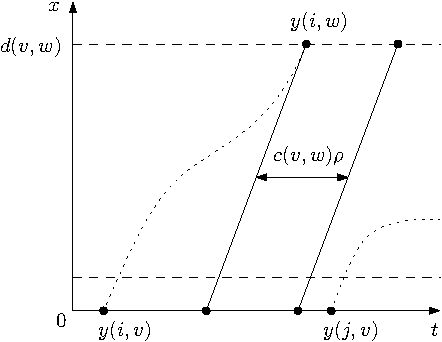
\includegraphics[width=0.8\textwidth]{figures/capacity_constraint.pdf}
  \caption{Illustration of the buffer constraint between $y(i, w)$ and
    $y(j, v)$. The slope of the two parallel lines is $v_{\max}$. The two dotted
    lines are examples of trajectories $x_{i}(t)$ and $x_{j}(t)$. The lower
    dashed line indicates $E_{r}(v)$ and the upper dashed line indicates
    $B_{r}(w)$.}\label{fig:buffer_constraints}
\end{figure}

\begin{proposition}
  When $y_{r}$ satisfies conjunctive
  constraints~\eqref{eq:conjunctive_constraints}, release constraints~\eqref{eq:release_constraints}, travel constraints \eqref{eq:travel_constraints} and buffer
  constraints \eqref{eq:buffer_constraints}, then $y_{r} \in \mathcal{S}_{r}$.
\end{proposition}

\begin{remark}
  It might be possible to relax the buffer constraints, i.e., there are
  situations in which vehicle $j$ is able to cross $v$ earlier.
\end{remark}


Given some crossing time schedule $y$ for vehicles $\mathcal{N}_{r}$, we show
how to compute trajectories by extending the \texttt{MotionSynthesize} procedure to
multiple \textit{checkpoints}
%
\begin{align*}
  \zeta = ((\tau_{1}, B_{1}), \dots, (\tau_{m}, B_{m})) ,
\end{align*}
where $\tau_{n}$ is a crossing time and $B_{n}$ is the beginning of the $n$th
intersection, measured along the path $V_{r}$ relative to $v_{r}(0)$.
%
Given the trajectory $x'$ of the vehicle ahead, the trajectory for a vehicle with
checkpoint sequence $\zeta$ is computed by the procedure
%
\begin{align*}
  \texttt{CheckpointTrajectory}(\zeta, x') := \\
  \text{arg min}_{x : [\tau_{1}, \tau_{m}] \rightarrow \mathbb{R}} \; &\int_{\tau_{0}}^{\tau_{m}} |x(t)|dt \\
  \text{ subject to } \; & \ddot{x}(t) = u(t) ,& \text{ for all } t \in [0, \tau_{m}] , \\
  & 0 \leq \dot{x}(t) \leq v_{\max} ,& \text{ for all } t \in [0, \tau_{m}] , \\
  & |u(t)| \leq a_{\max} ,& \text{ for all } t \in [0, \tau_{m}] , \\
  & x'(t) - x(t) \geq L ,& \text{ for all } t \in [0, \tau_{m}] , \\
  & x(\tau_{n}) = B_{n} ,& \text{ for all } n = 1, \dots, m , \\
  & \dot{x}(\tau_{n}) = v_{\max} ,& \text{ for all } n = 1, \dots, m .
\end{align*}


\bibliography{references}
\bibliographystyle{ieeetr}

\end{document}
